\chapter{Experiments and Results}

% **************************** Define Graphics Path **************************
\ifpdf
    \graphicspath{{Chapter3/Figs/Raster/}{Chapter3/Figs/PDF/}{Chapter3/Figs/}}
\else
    \graphicspath{{Chapter3/Figs/Vector/}{Chapter3/Figs/}}
\fi
This chapter discusses the experiments done to evaluate the techniques described in the previous chapter. The speech samples used were taken from the TIMIT database \cite{TIMIT}. 40 different sentences were chosen from the database for this purpose. These were each sampled at 16kHz. To add reverberation to these clean speech signals, room impulse responses provided by the REVERB 2014 challenge were used. In particular 3 room impulse responses from 3 rooms each with reverberation times (t60) 0.25s, 0.5s and 0.7s were used. Although these responses were recorded using multiple channels, only one channel per room impulse response was used here since these techniques apply to single channel dereverberation.   Reverberant speech signals we generated by convolving clean speech signals with these room impulse responses. MATLAB was used to implement all the techniques. The code for the NMFD algorithm discussed in Section 3.1 was otained from \cite{gamma}. All other techniques have been implemented by us. 
For converting time domain signals into magnitude spectrograms, a sliding square root hann window \cite{moham} length 64ms  was used with an overlap of 16ms between frames.

All the techniques will be quantitatively compared on their performances in dereverberating speech recordings. The techniques are applied to the magnitude spectrogram of the reverberant speech input to obtain a clean magnitude spectrogram. This spectrogram, using the phase information of the input signal is then converted to the time domain. 
To quantify the performance, the following key objective measures are used - 
\begin{enumerate}
\item \textbf{Perceptual evaluation of speech quality (PESQ)} \\
PESQ is a widely used measure to judge the quality of speech as heard by humans. It uses the clean speech as a reference to score the output speech on its quality. A higher score indicates better quality of speech. The performance of a dereverberation technique is good if the PESQ score of the output is more than that of the input.
\item \textbf{Cepstral distortion(CD)} \\
Mel-cepstral coefficients are perhaps the most frequently used features for speech recognition. A distortion in the cepstral coefficients can thus significantly decrease performance in recognition. Therefore, an important measure of how much a speech signal has been affected by reverberation is the amount of distortion introduced in the cepstral coefficients. A quantitative measure of this is the Cepstral distortion. 

\end{enumerate}


\section{Dereverberation using NMFD}

For this technique, discussed in Section 3.1, the multiplicative updates according to (3.4) and (3.5) were carried out for 20 iterations. $\lambda$ , the sparsity parameter was fixed to be $\sum_{k,t}Y \times 10^{-8}$ as suggested in \cite{naka}. However experimentally, we found that having a sparsity constraint did not help in improving algorithm performance.
Initially, the clean speech estimate, $X$ was set to be equal to $Y$ and $H$ was initialized as a linearly decaying filter.
The length of the filter, was fixed at $L=11$ frames in the spectrogram, i.e. a time domain span of 352ms. The average improvements in the PESQ scores and the CD scores are shown in Figures 4.10 and 4.11. Figures 4.2, 4.3 and 4.4 shows the spectrogram of the reverberant speech, the output clean speech and the output filter, $H$. In the output spectrogram, smearing of the features is reduced, specially in the sparser regions.
\begin{figure}
\centering
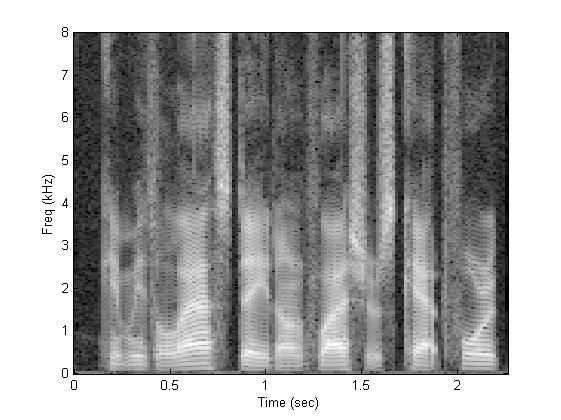
\includegraphics[scale=0.8]{clean}
\caption{Clean speech Spectrogram }
\end{figure}

\begin{figure}
\centering
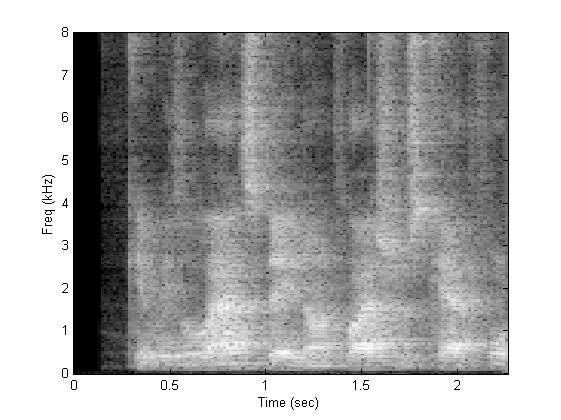
\includegraphics[scale=0.8]{input_normal}
\caption{Reverberated Spectrogram }
\end{figure}
\begin{figure}
\centering
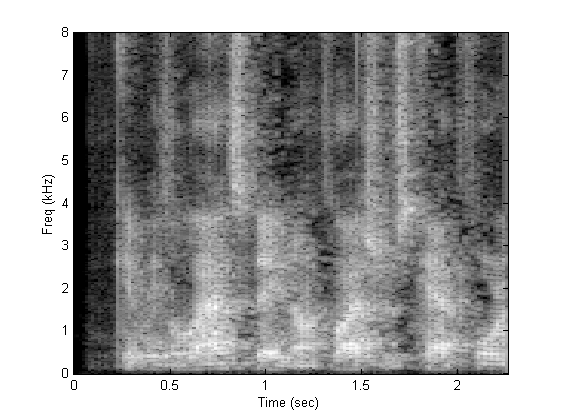
\includegraphics[scale=0.8]{output_normal}
\caption{Dereverberated Spectrogram }
\end{figure}
\begin{figure}
\centering
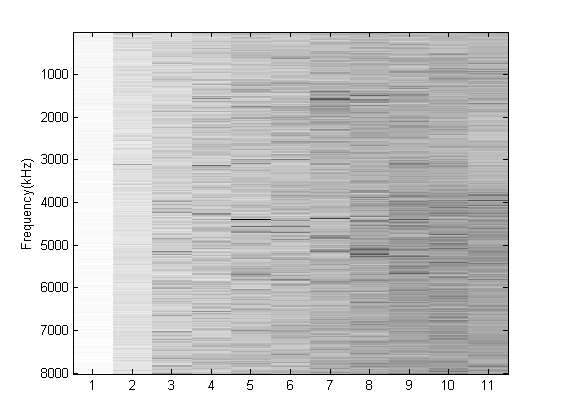
\includegraphics[scale=0.8]{H_normal}
\caption{Recovered H filter. the filter length was chosen to be 11 frames. The sum of each of the rows of this H matrix is 1.  The X axis represents the frame numbers, where each frame is temporally equivalent to 32ms.}
\end{figure}
The recovered H filter, in Figure 4.4, is displayed using a decibel scale to make it seem more uniform. The initial values of the sub-band filters are much larger than the later values by an order of magnitude. To observe the variation of the performance of the algorithm with varying lengths for the filter, H for each RIR, the length of the filter was varied from 128ms to 640ms. The results are shown in Figure 4.5

\begin{figure}
\centering
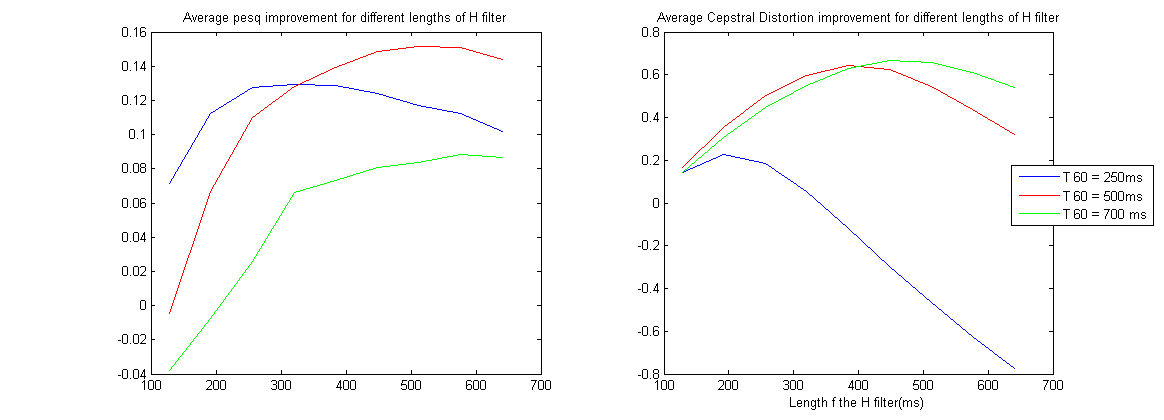
\includegraphics[scale=0.6]{normal_performance}
\caption{Varying the filter length for different T60. Higher T60 values had a higher performance for longer lengths of the H filter}
\end{figure}
It is clear from the results in Figure 4.5, that the length of the filter H, has some correlation to the degree of reverberation in the recorded speech signals. For a higher T 60, the PESQ and Cepstral Distortion are best for greater lengths of $H$ when the T 60 is higher and for lower lengths of $H$ for lower T 60 values. This makes intuitive sense since a larger T 60 value implies that the effect of reverberation on a frame affects frames further in the magnitude spectrogram than it would if the T60 was lower.
\section{Activation Deconvolution}
The activation deconvolution technique was applied over the same 40 sentences from TIMIT database using the same updates used in (3.4) and (3.5) for NMFD. The number of basis chosen was $R = 20$ and the length of the filter h(t) in Equation 3.6 was chosen to be $L=11$ frames, which translates to 352ms. The output speech was measured for improvement in PESQ, Cepstral Distortion and SRMR scores. The mean results are shown in Figure \ref{act_decon_results}. \\
It can be seen that the cepstral distortion scores have improved for T60s 500ms and 700ms. PESQ score has only increased for T60 500ms. There are audible artifacts in the output sound as well. We infer that the effectof reverberation on the activation vectors has not been modelled appropriately through this approach. A better model for this is needed.

\begin{figure}
\centering
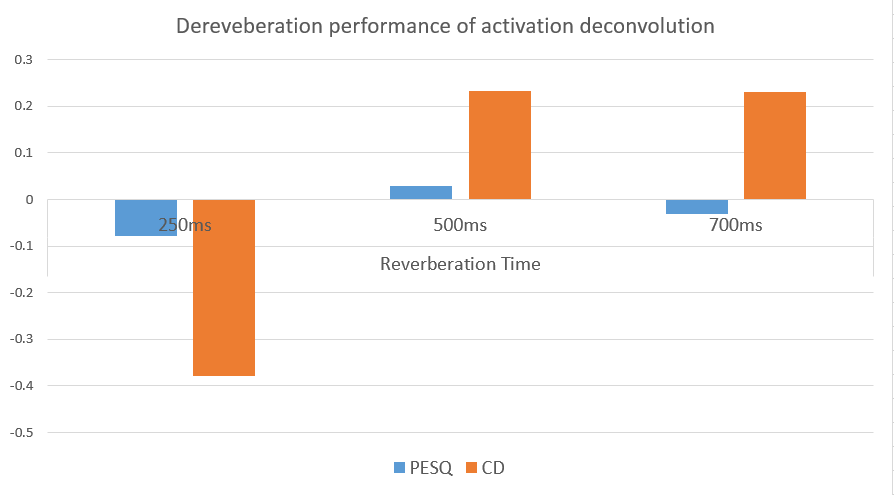
\includegraphics[scale=0.6]{act_decon_results}
\caption{Results for the Activation deconvolution technique. The improvements in PESQ and CD scores for different levels of reverberation are shown. Note that a negative value indicates that the output is worse than the reverberant input for the particular measure}\label{act_decon_results}
\end{figure}
\section{NMFD using NMF model for speech}
Including the NMF model for speech, the updates given by (3.8), (3.9) and (3.10), were carried out for 20 iterations. The number of basis vectors used to represent the speech signals, $R$, used was 10. Having more number for basis vectors gave very marginal increase in performance while adding to the computation time. This is clear from the increase in the mean PESQ and CD performance improvement across the 40 senteneces from TIMIT, shown in Figures 4.7 and 4.8. The sparsity parameter, $\lambda$ was the same as in the previous section. The result for this algorithm are shown in Figure 4.9, for one sentence from the TIMIT database.

\begin{figure}
\centering
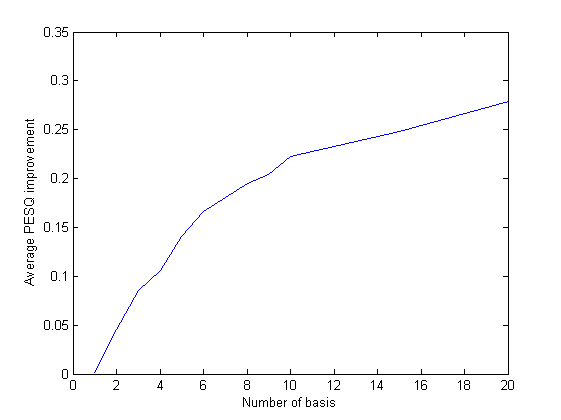
\includegraphics[scale=0.8]{pesq_no_bases}
\caption{Number of basis on performance}
\end{figure}


\begin{figure}
\centering
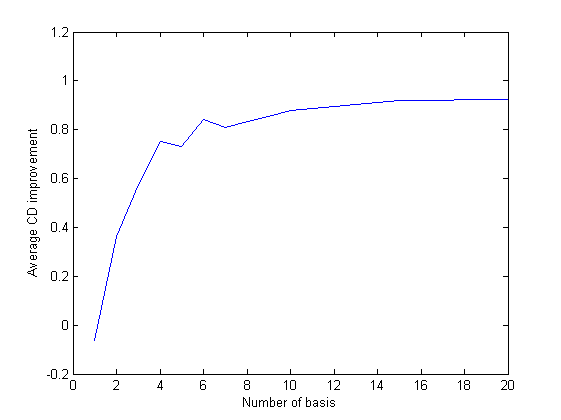
\includegraphics[scale=0.8]{cd_no_bases}
\caption{Number of basis on performance. Both figure 4.7 and 4.8 unequivocally suggest that more basis vectors in the NMF decomposition will provide better results for dereverberation. However, the marginal increase in performance after a certain number of basis is minimal}
\end{figure}
\begin{figure}
\centering
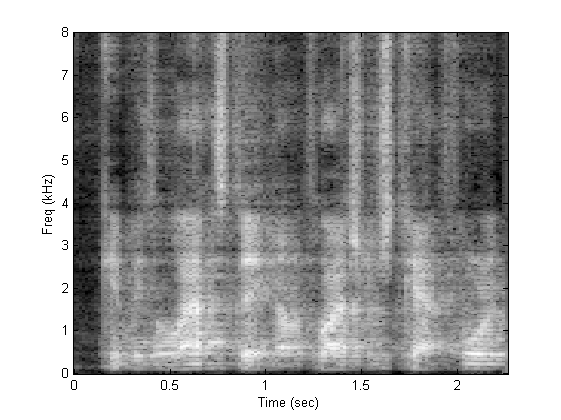
\includegraphics[scale=0.8]{output_NMF}
\caption{Output spectrogram for NMFD with NMF model}
\end{figure}

A comparative analysis is done, and the results reproduced in Figures 4.10 and 4.11 to show the improvements gained in the PESQ scores and Cepstral Distortion Scores by introducing the NMF model for speech. It can be seen that significant improvement in PESQ scores was observed. The improvement in the Cepstral distortion scores was not significant.
\begin{figure}
\centering
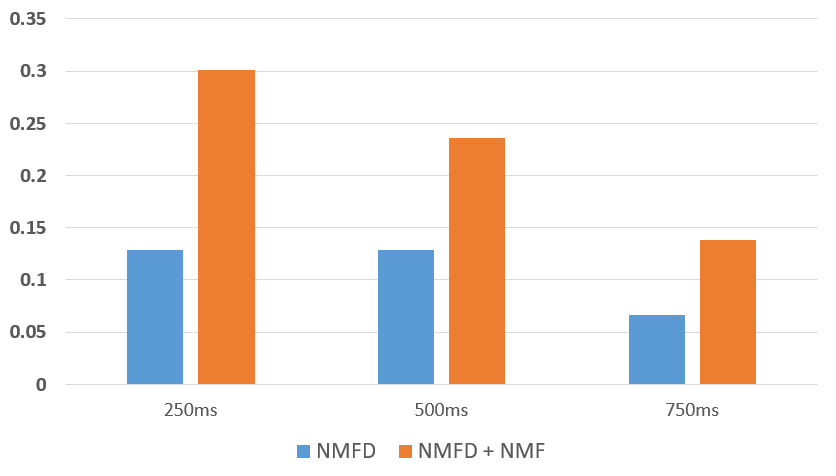
\includegraphics[scale=0.6]{pesq_comp}
\caption{Output for NMFD with NMF model}
\end{figure}
\begin{figure}
\centering
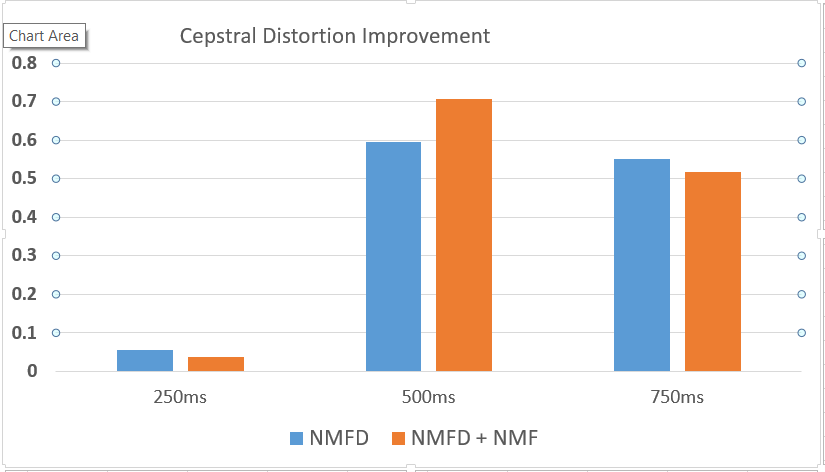
\includegraphics[scale=0.6]{cd_comp}
\caption{Output for NMFD with NMF model}
\end{figure}

\section{Frame stacked model}
The frame stacked model discussed in Section 3.4.1, aims to exploit the temporal continuity of speech through stacking the magnitude domain spectrogram in a sequential manner. The updates for this model are as given in (3.12). The temporal context to use for stacking, quantified by the variable, $T_{stack}$ . These updates are given 20 iteration to converge and then, the gain function, $G$ is calculated using (3.13) is calculated. 

The results for the stacked model were not found to be promising. In fact, performance gets worse even if $T_{stack} = 2$. It does not outperform the simple NMF model for any of the reverberant scenarios, as far as improving the PESQ and the Cepstral Distortion scores are concerned. This agrees with the results in literature where this model has not been able to outperform the simple NMF model for speech.

\section{NMFD and the Convolutive NMF model }
This section discusses the results of NMFD with the Convolutive NMF model used for speech. The modified updates for this approach are given in (3.14). This approach has not yet been presented in any literature to the best of our knowledge, although \cite{baby} has used the convolutive NMF model as part of a supervised approach. The updates are derived on similar lines as the stacked model. Again, of major importance is the temporal context used. The length of the convolutive basis, $T_{base}$, has a major influence on the algorithms performance. 
\begin{figure}
\centering
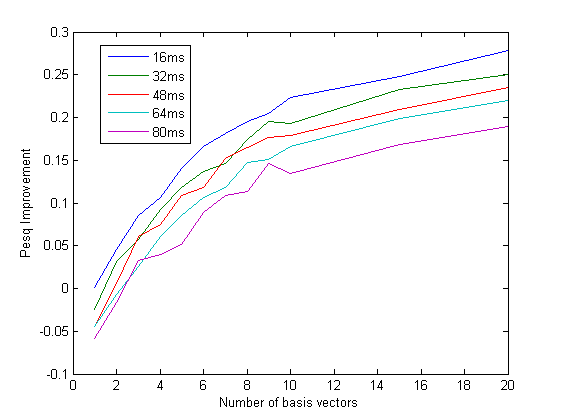
\includegraphics[scale=0.6]{bases_cnmf_pesq}
\caption{PESQ score versus number of bases(x-axis) and length of bases(plot lines).Figures 4.12 and 4.13 show the improvement in performance with increasing number of basis vectors, across different basis lengths. A basis length of 16ms, which is equivalent to one frame, implies a regular NMF. All other multiples of 16ms correspond to convolutive basis vectors. Each plot line corresponds to a fixed length of the convolutive basis}
\end{figure}

\begin{figure}
\centering
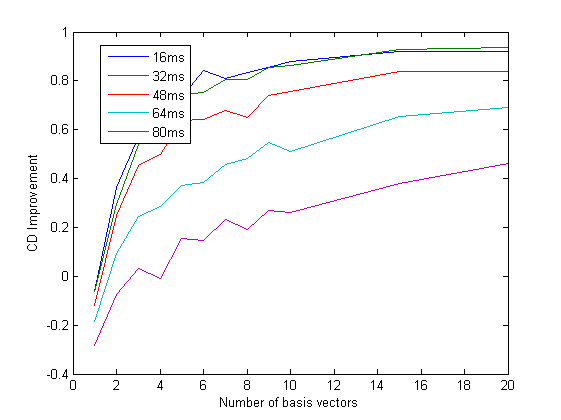
\includegraphics[scale=0.6]{bases_cnmf_cd}
\caption{CD scores. Figures 4.12 and 4.13 show the improvement in performance with increasing number of basis vectors, across different basis lengths. A basis length of 16ms, which is equivalent to one frame, implies a regular NMF. All other multiples of 16ms correspond to convolutive basis vectors. Each plot line corresponds to a fixed length of the convolutive basis}
\end{figure}

It is clear from Figures 4.12 and 4.13 that increasing the length of the basis, $T_{base}$ has a detrimental impact on the performance of the algorithm, both in terms of PESQ scores as well as Cepstral Distortion scores but more number of bases is beneficial in both measures. Each plot line, corresponding to a longer basis vector is lower than that of one with a shorter one. It can be concluded that Convolutive NMF representation of speech does not help in increasing dereverberation performance.

\section{Discussion}
As per the measures, it is clear that NMFD, with an NMF representation of speech is the best among all techniques for dereverberation. Our hypothesis as to why it is so is that by applying the sparsity constraint on the activations, rather than on the whole spectrogram, as in NMFD, it has provided a better model for speech magnitude spectrograms. Also, activation deconvolution, although does not do as well as NMFD provided an alternative approach to tackle dereverberation in the magnitude spectrogram domain. The approach, as it is now, also introduces artifacts in the output speech. 
As far as exploiting the temporal dynamics of speech is concerned, neither the frame stacked model, nor the convolutive model improve the performance of the algorithm as far as the objective measures are concerned. 
The qualitative results obtained in this chapter corroborate with the existing literature \cite{moham} although the exact improvements in objective measures obtained are still not as high. This might be due to different datasets used or difference in implementation details. The summary of all the results is given in Table 4.1 and 4.2

\begin{table}
\centering
\caption{Summary of the PESQ improvement by discussed techniques}
\label{my-label}
\begin{tabular}{llll}
                             & \multicolumn{3}{c}{\textbf{T60}} \\
\textbf{Technique}           & 250ms     & 500ms     & 750ms    \\
NMFD                         & 0.1291    & 0.1283    & 0.0662   \\
NMFD + NMF                   & 0.301259  & 0.235671  & 0.138228 \\
Stacked model (T\_stack = 3) & 0.135805  & 0.192561  & 0.094765
\end{tabular}
\end{table}

\begin{table}[]
\centering
\caption{Summary of the PESQ improvement by discussed techniques}
\label{my-label}
\begin{tabular}{llll}
                             & \multicolumn{3}{c}{\textbf{T60}} \\
\textbf{Technique}           & 250ms     & 500ms     & 750ms    \\
NMFD                         & 0.0552    & 0.5963    & 0.5516   \\
NMFD + NMF                   & 0.0381    & 0.7068    & 0.5180   \\
Stacked model (T\_stack = 3) & 0.0312    & 0.4021    & 0.4974  
\end{tabular}
\end{table}